\chapter{Kết quả và đánh giá}
\label{ch:ketqua}

\begin{muctieu}
Chương này đối chiếu mục tiêu, trình bày audit dữ liệu, đánh giá model trên
tập Test sạch và phân tích những hạn chế của sản phẩm.
\end{muctieu}

\newcommand{\EvalTotal}{5.014}
\newcommand{\EvalCorrect}{4.690}
\newcommand{\EvalAccuracy}{93,54\%}
\newcommand{\EvalMacroPrecision}{94,00\%}
\newcommand{\EvalMacroRecall}{93,41\%}
\newcommand{\EvalMacroFOne}{93,68\%}
\newcommand{\EvalMeanConfidence}{93,30\%}
\newcommand{\EvalMeanMs}{1410,0}
\newcommand{\EvalPPercentileMs}{1406,8}


\section{Mức độ hoàn thành mục tiêu}

Ứng dụng đã hoàn thiện luồng Flutter--FastAPI, nhận diện ảnh bằng model 38
nhãn, tìm kiếm và hiển thị 38 công thức có nguồn. Các chức năng đăng ký,
đăng nhập, chế độ khách, yêu thích, lịch sử, phản hồi và sửa tên được tích
hợp. Backend có migration, audit, importer và tài liệu OpenAPI. Như vậy năm
nhóm mục tiêu sản phẩm ở Chương~\ref{ch:modau} đã được hiện thực; phạm vi
production nhiều người dùng vẫn là hướng phát triển.

\section{Kết quả dữ liệu công thức}

\begin{table}[htbp]
\centering
\caption{Thống kê kho công thức sau audit.}
\label{tab:recipe-audit}
\begin{tabular}{>{\bfseries}l r}
\toprule
Thuộc tính & Kết quả \\
\midrule
Món đã xuất bản & 38/38 \\
Ảnh có metadata đầy đủ & 38/38 \\
Nguyên liệu & 348 \\
Bước thực hiện & 205 \\
Nguồn tham khảo & 85 \\
Công thức dịch nguồn mở & 8 \\
Công thức biên soạn đối chiếu & 30 \\
\bottomrule
\end{tabular}
\end{table}

Audit xác nhận mỗi món có thời gian sơ chế, nấu, tổng thời gian, khẩu phần,
ít nhất một nguyên liệu và một bước. Ảnh local giải mã được và metadata khớp
manifest. Việc tách catalog nguồn mở với catalog biên soạn giúp hiển thị đúng
nguồn gốc nội dung và phạm vi giấy phép.

\section{Audit và làm sạch 30VNFoods}

Dataset gốc có 25.136 ảnh JPG thuộc 30 lớp: 17.581 Train, 2.515 Validate và
5.040 Test. Tất cả ảnh đều được Pillow đọc thành công. Audit SHA-256 phát
hiện 63 nhóm trùng, 40 nhóm đi qua nhiều split và 38 nhóm có cùng ảnh nhưng
khác nhãn. Chính sách làm sạch giữ một bản cho nhóm trùng cùng nhãn, ưu tiên
Test rồi Validate và Train; nhóm mâu thuẫn nhãn bị loại hoàn toàn.

Manifest sạch còn 25.032 ảnh: 17.515 Train, 2.503 Validate và 5.014 Test như
Hình~\ref{fig:dataset-splits}. Dữ liệu raw không bị sửa.

\begin{figure}[htbp]
\centering
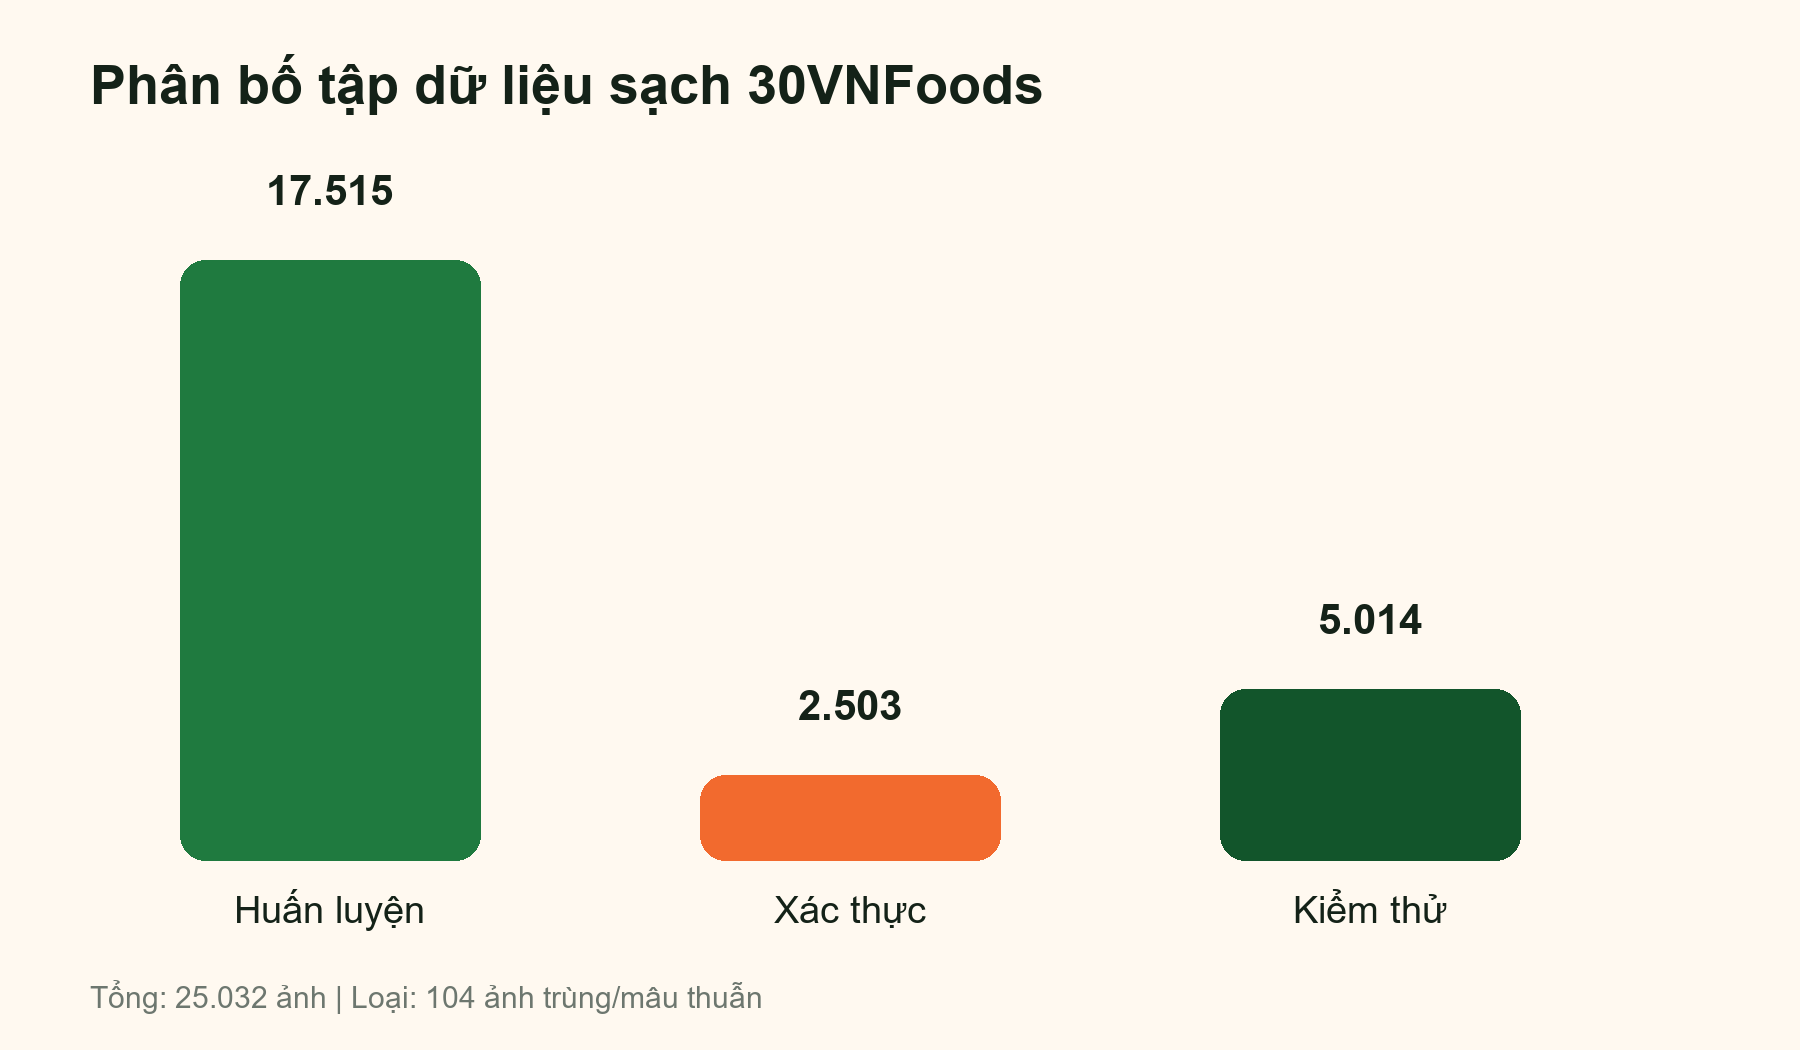
\includegraphics[width=0.88\textwidth]{figs/charts/dataset-splits.png}
\caption{Phân bố các split sau khi loại ảnh trùng và mâu thuẫn.}
\label{fig:dataset-splits}
\end{figure}

Số ảnh giữa các lớp không hoàn toàn cân bằng. Hình~\ref{fig:dataset-classes}
cho thấy Bún bò Huế, Bánh mì và Bánh xèo có nhiều mẫu hơn một số lớp như Bánh
pía hoặc Bánh chưng. Vì vậy báo cáo sử dụng thêm macro F1 thay vì chỉ đọc
accuracy.

\clearpage
\thispagestyle{dau}
\vspace*{\fill}
\begin{center}
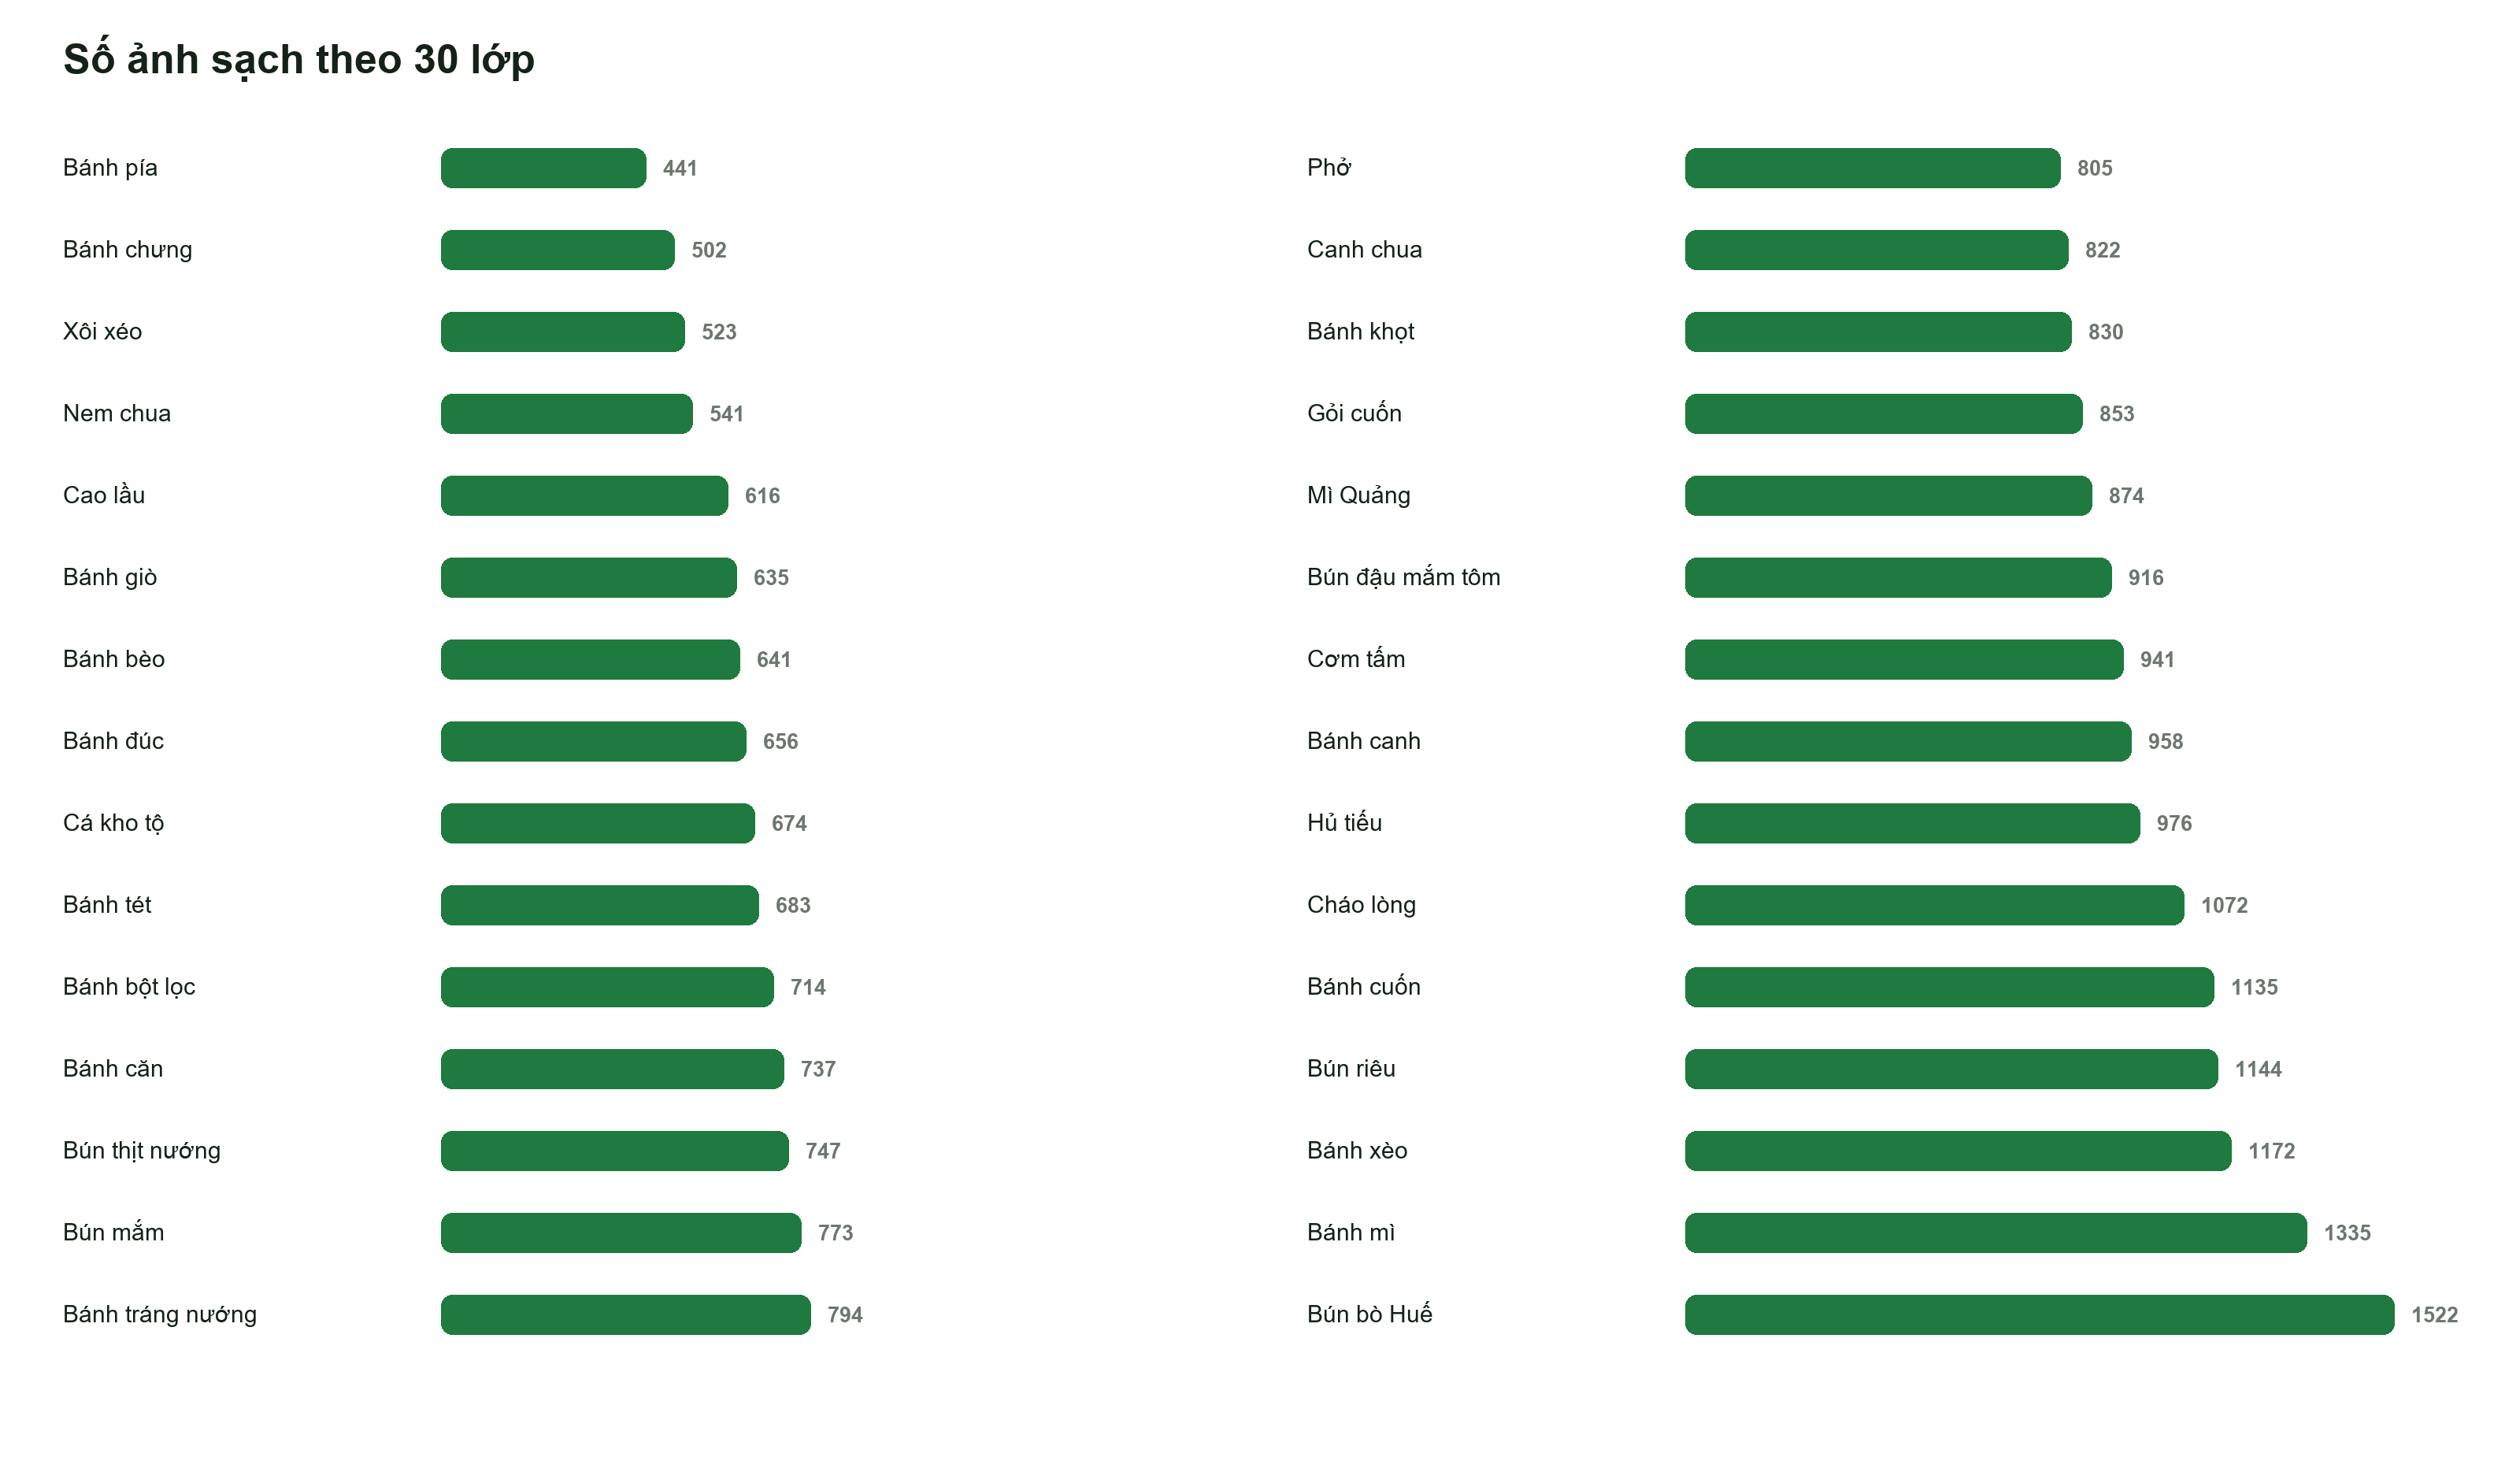
\includegraphics[width=\textwidth]{figs/charts/dataset-classes.png}
\dauFigureCaption{Số ảnh sạch theo từng lớp trong toàn bộ ba split.}{fig:dataset-classes}
\end{center}
\vspace*{\fill}
\clearpage

\section{Kết quả đánh giá model}

Model được chạy trên toàn bộ \EvalTotal{} ảnh của manifest Test sạch. Nhãn
dataset được chuẩn hóa bằng cùng module alias với backend. Một dự đoán chỉ
được tính đúng khi tên chuẩn Top~1 trùng ground truth. Các dự đoán rơi vào
tám lớp ngoài phạm vi 30VNFoods vẫn được tính là sai.

\begin{table}[htbp]
\centering
\caption{Kết quả đánh giá trên tập Test sạch.}
\label{tab:model-metrics}
\begin{tabular}{>{\bfseries}l r}
\toprule
Độ đo & Giá trị \\
\midrule
Số ảnh đánh giá & \EvalTotal \\
Số dự đoán đúng & \EvalCorrect \\
Accuracy Top~1 & \EvalAccuracy \\
Macro Precision & \EvalMacroPrecision \\
Macro Recall & \EvalMacroRecall \\
Macro F1 & \EvalMacroFOne \\
Confidence trung bình & \EvalMeanConfidence \\
Thời gian trung bình/ảnh & \EvalMeanMs{} ms \\
P95 thời gian/ảnh & \EvalPPercentileMs{} ms \\
\bottomrule
\end{tabular}
\end{table}

Các con số trong Bảng~\ref{tab:model-metrics} là kết quả chạy tại máy thử
nghiệm, không phải số liệu do model card công bố. Thời gian/ảnh được chia đều
theo batch và phụ thuộc thiết bị, backend, batch size và trạng thái bộ nhớ.

\IfFileExists{figs/charts/per-class-metrics.png}{
\clearpage
\thispagestyle{dau}
\vspace*{\fill}
\begin{center}
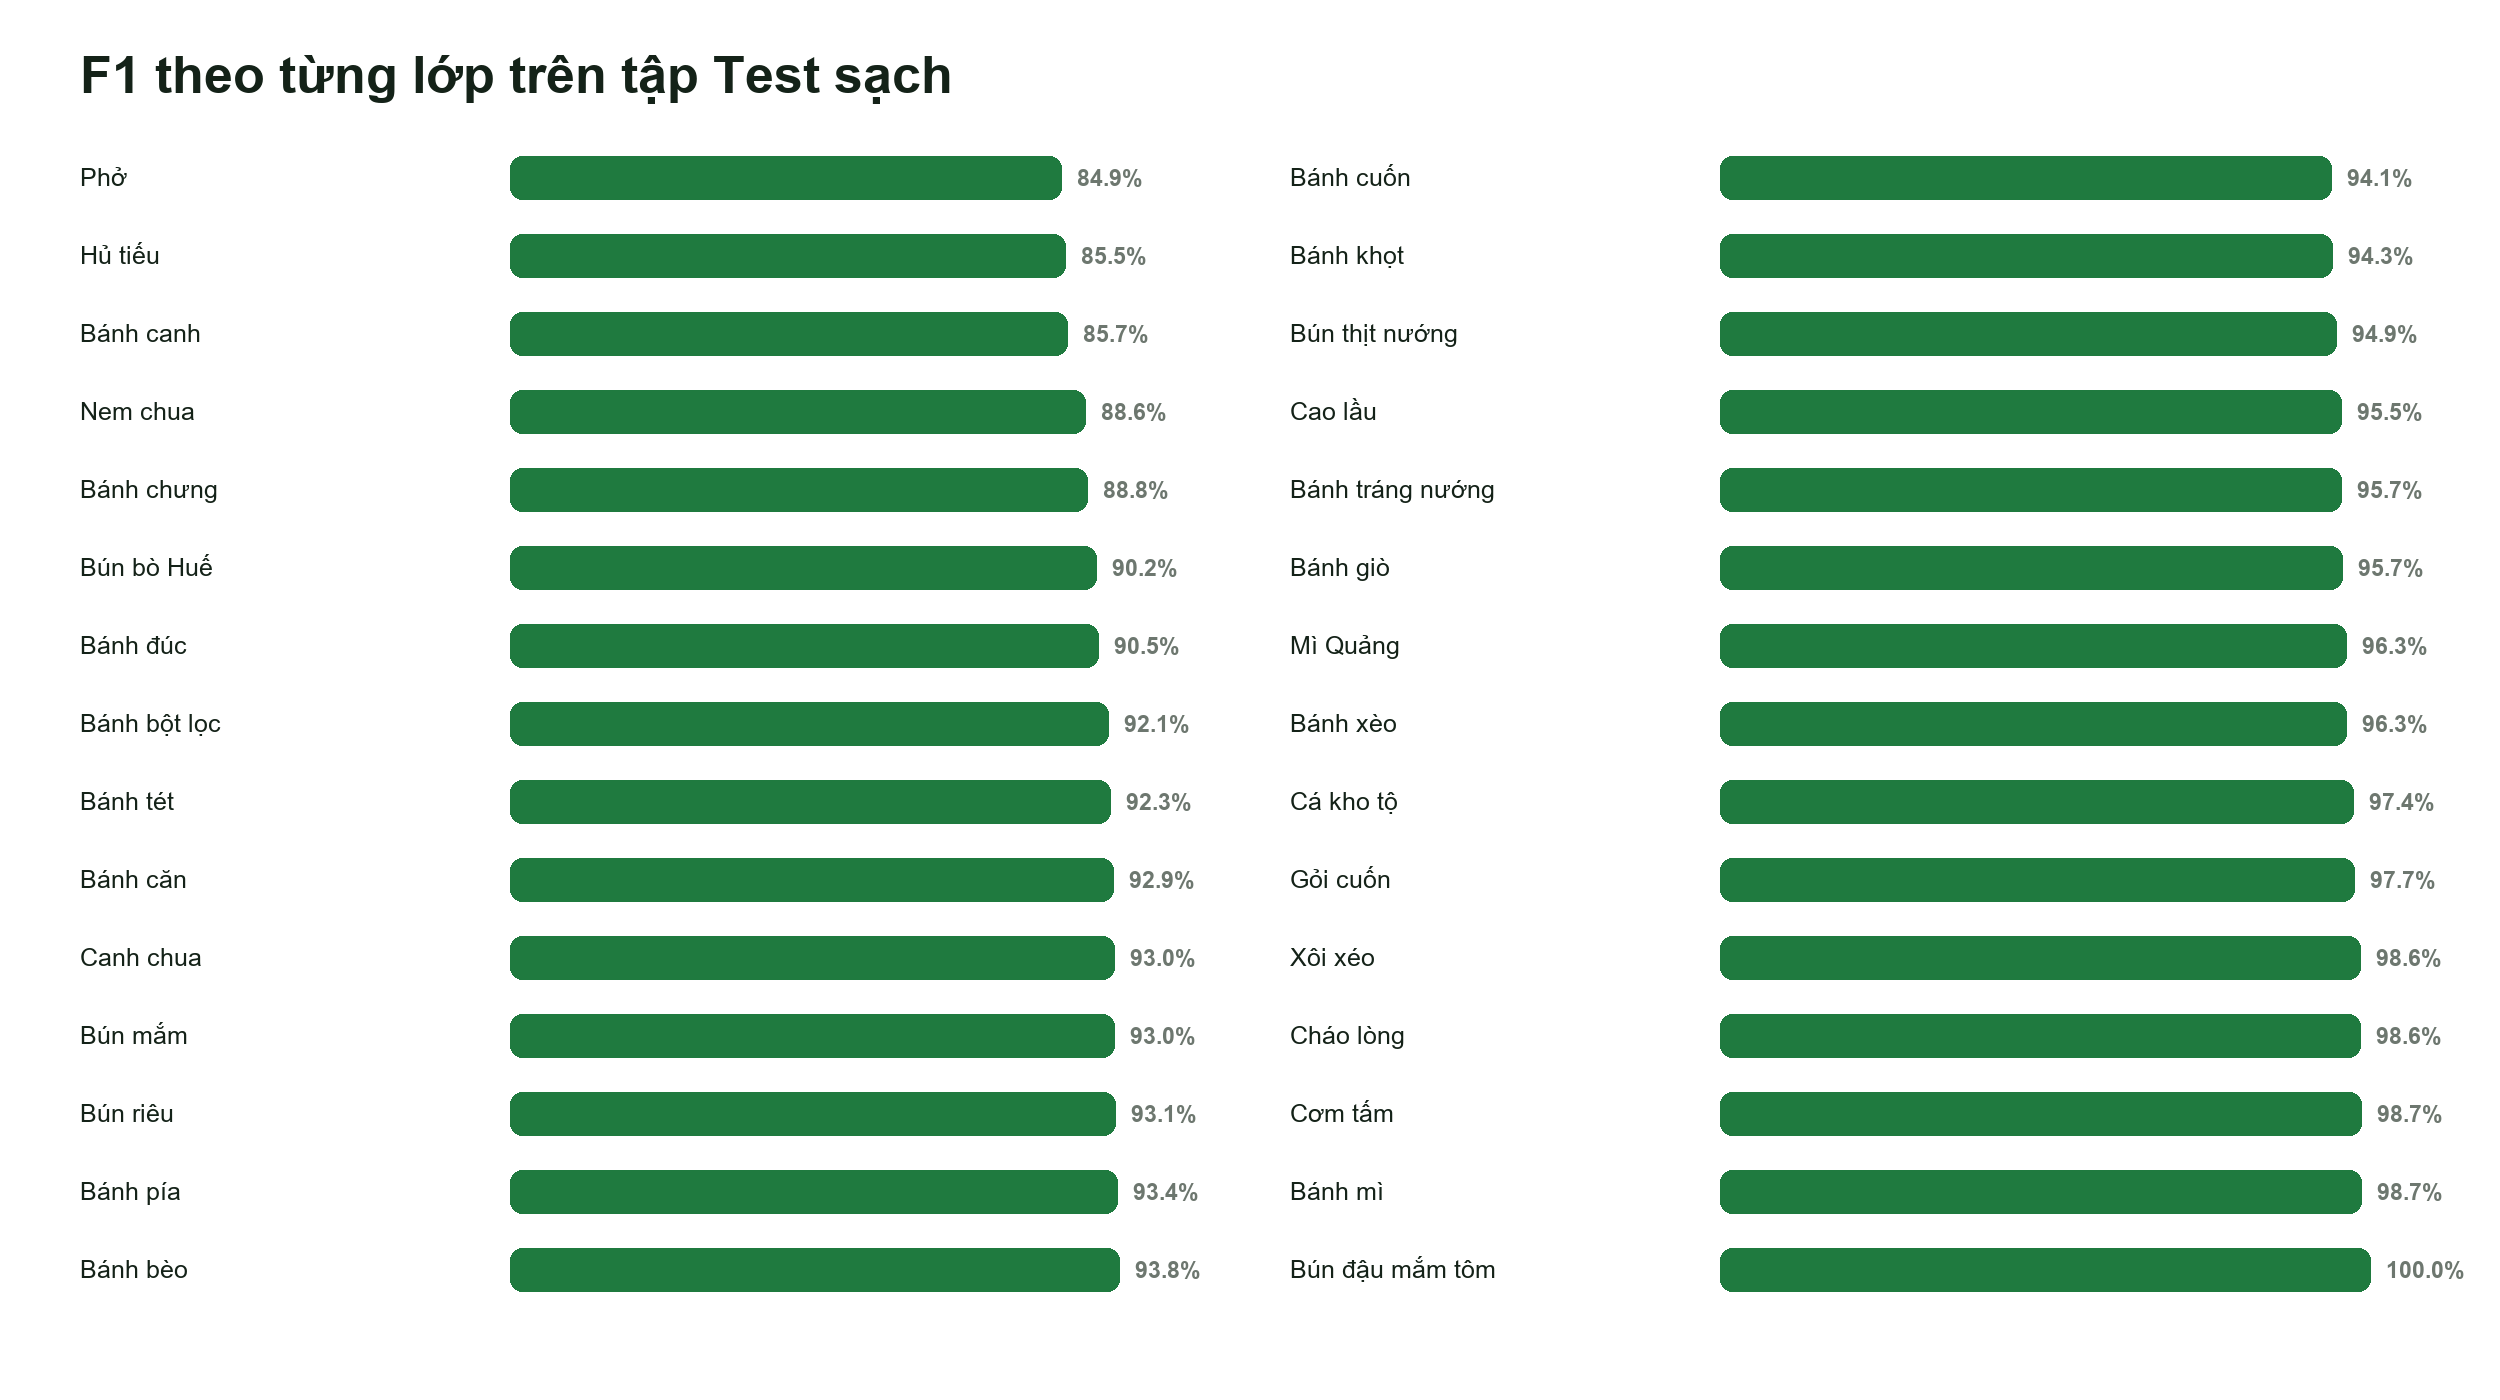
\includegraphics[width=\textwidth]{figs/charts/per-class-metrics.png}
\dauFigureCaption{F1 theo từng lớp trên tập Test sạch.}{fig:per-class-metrics}
\end{center}
\vspace*{\fill}
\clearpage
\thispagestyle{dau}
\vspace*{\fill}
\begin{center}
\IfFileExists{figs/charts/confusion-matrix.png}{%
  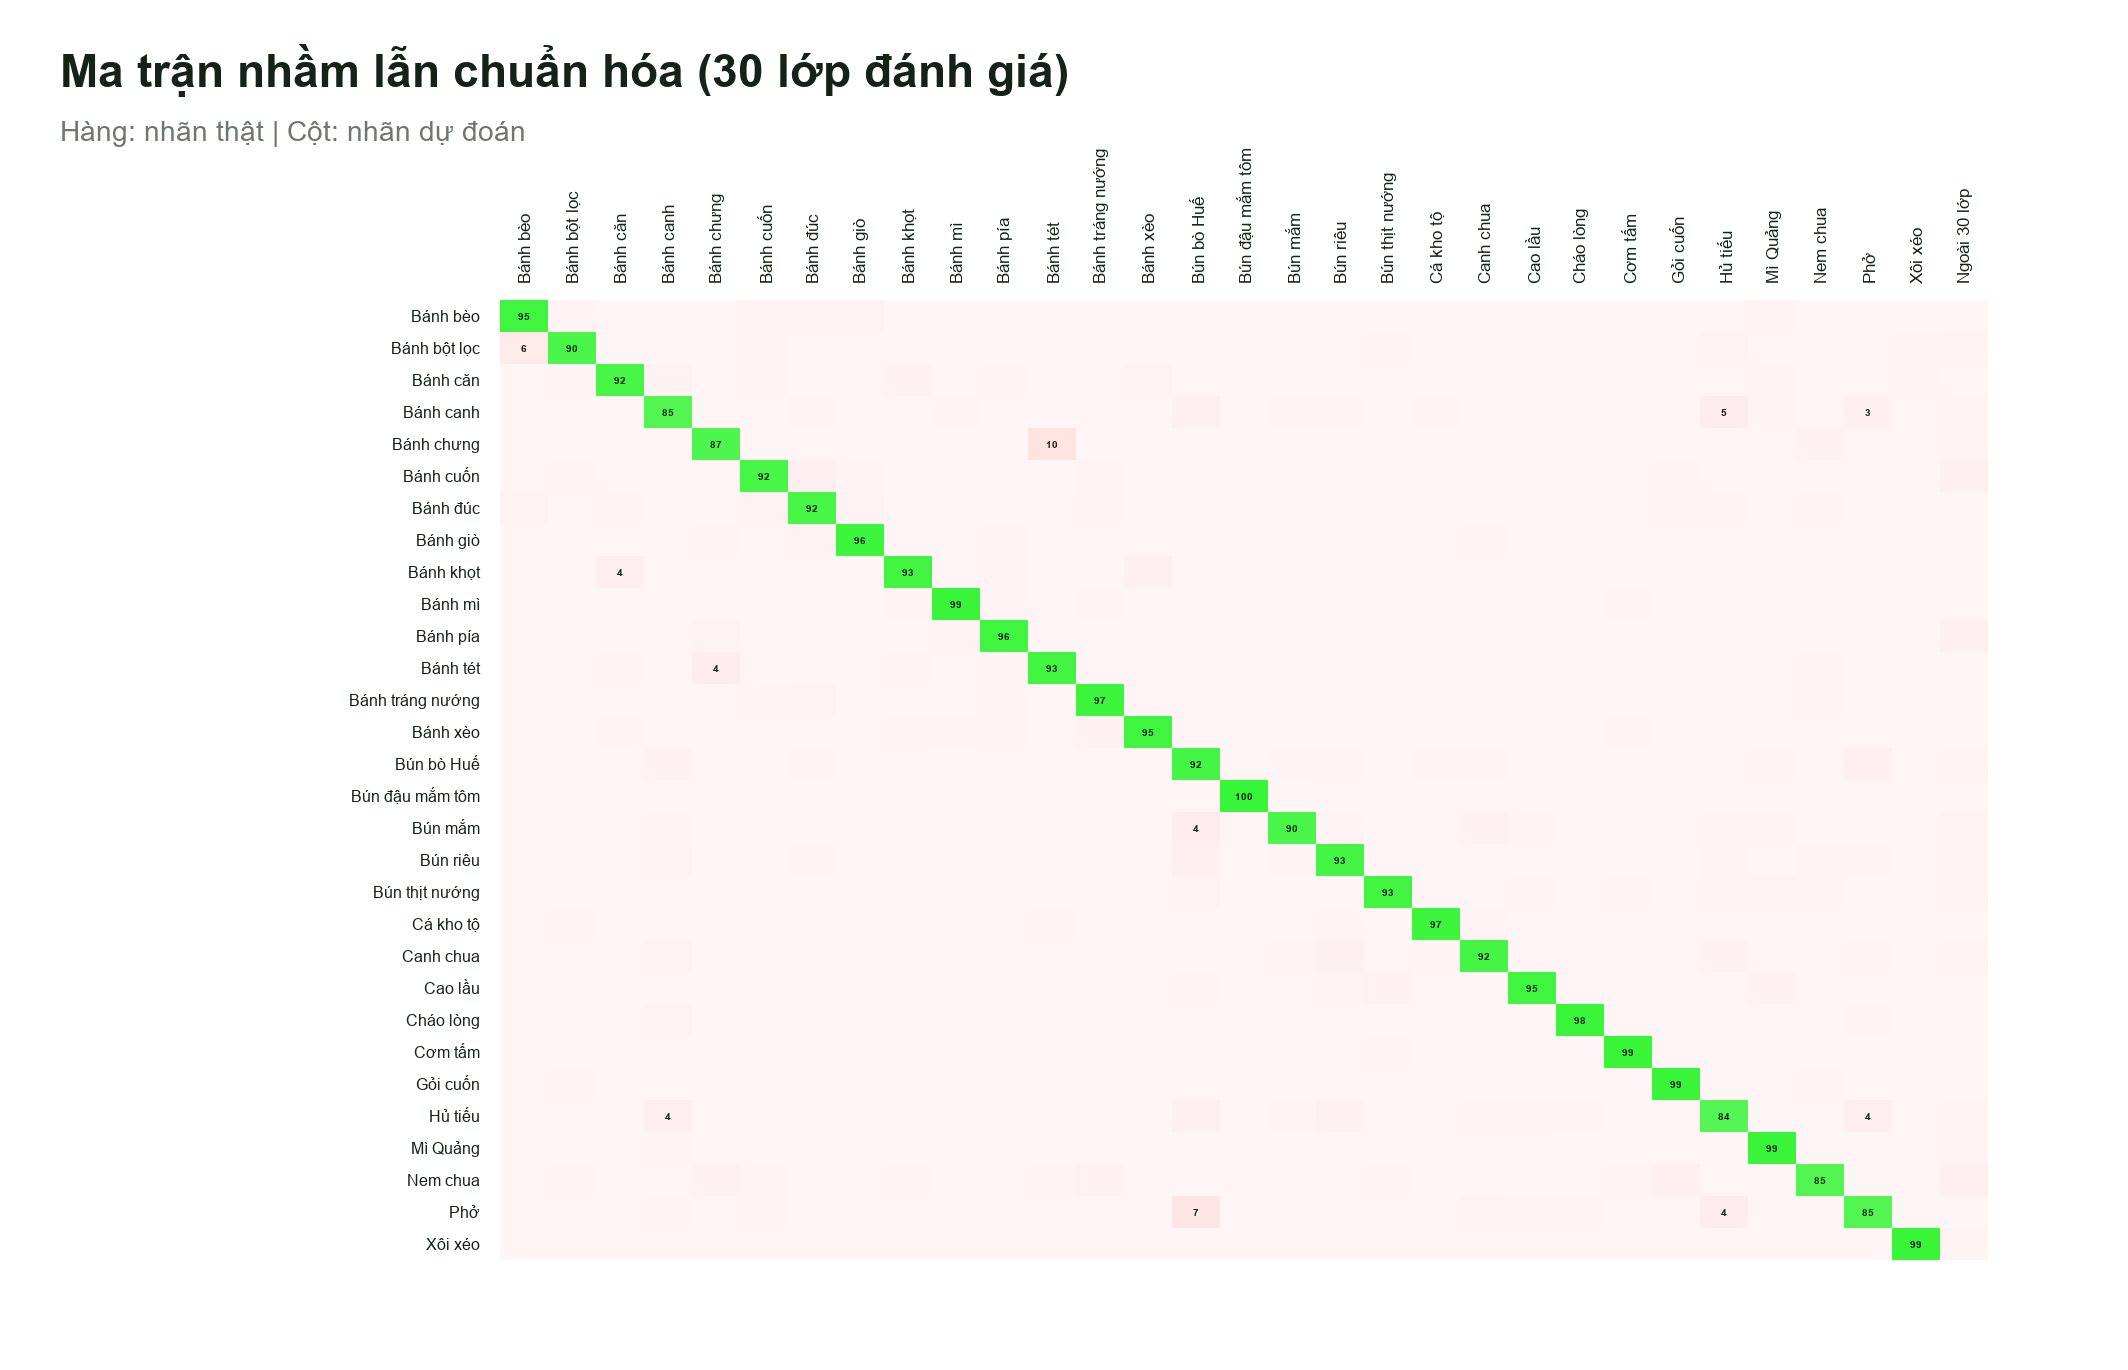
\includegraphics[width=\textwidth,height=0.72\textheight,keepaspectratio]{figs/charts/confusion-matrix.png}
  \dauFigureCaption{Ma trận nhầm lẫn chuẩn hóa; tám nhãn ngoài dataset được gộp thành một cột.}{fig:confusion-matrix}%
}{}
\end{center}
\vspace*{\fill}
\clearpage
}{}

\IfFileExists{evaluation/top-confusions.tex}{\begin{table}[htbp]
\centering
\caption{Các cặp nhầm lẫn xuất hiện nhiều nhất.}
\label{tab:top-confusions}
\begin{tabular}{>{\bfseries}l l r}
\toprule Nhãn thật & Dự đoán & Số ảnh \\
\midrule
Phở & Bún bò Huế & 12 \\
Bánh chưng & Bánh tét & 10 \\
Bánh canh & Hủ tiếu & 9 \\
Bún bò Huế & Phở & 9 \\
Bánh bột lọc & Bánh bèo & 8 \\
Hủ tiếu & Phở & 7 \\
Hủ tiếu & Bánh canh & 7 \\
Bánh canh & Phở & 6 \\
Bánh cuốn & Bánh đúc & 6 \\
Bánh khọt & Bánh căn & 6 \\
\bottomrule
\end{tabular}
\end{table}
}{}

\section{Kết quả kiểm thử phần mềm}

\IfFileExists{evaluation/test-status.tex}{\begin{table}[htbp]
\centering
\caption{Kết quả kiểm thử và build tại lần nghiệm thu báo cáo.}
\label{tab:test-status}
\begin{tabularx}{\textwidth}{>{\bfseries}p{4.1cm} p{2.3cm} X}
\toprule
Hạng mục & Trạng thái & Kết quả \\
\midrule
Backend pytest & PASS & 24 test, 48 subtest; 2 cảnh báo deprecation; 12,24 giây \\
Flutter analyze & PASS & Không phát hiện issue; 53,4 giây \\
Flutter test & PASS & 21/21 test; khoảng 5 giây \\
Audit công thức & PASS & 38 món, 38 ảnh, metadata đầy đủ, không có lỗi \\
Build APK debug & PASS & Sinh \code{mobile/build/}\\\code{app/outputs/}\\\code{flutter-apk/}\\\code{app-debug.apk} \\
Android Emulator & CHƯA THỬ LẠI & Có ảnh nghiệm thu luồng camera, Top~1 và mở công thức; chưa chạy lại thao tác tương tác trong phiên tạo báo cáo \\
\bottomrule
\end{tabularx}
\end{table}

Backend test phát sinh hai cảnh báo không làm test thất bại: TestClient của
Starlette sẽ chuyển sang \code{httpx2}, và cấu hình Alembic chưa khai báo
\code{path\_separator}. APK build có cảnh báo phiên bản SDK XML giữa Android
Studio và command-line tools nhưng Gradle vẫn kết thúc với mã thoát 0.
}{
\begin{luuy}
Kết quả kiểm thử tự động chưa được ghi nhận bằng mã thoát rõ ràng. Không được
tuyên bố PASS trước khi chạy lại và lưu log.
\end{luuy}}

Audit công thức đã chạy thành công và trả \code{ok=true}, 38 món published,
38 ảnh và 38 bản ghi metadata hoàn chỉnh. Kiểm thử phần mềm được chạy tuần
tự để tránh xung đột cache; trạng thái trong bảng được lấy từ log cùng lần
nghiệm thu báo cáo.

\section{Bàn luận}

Kết quả cần được đọc trong bối cảnh 30VNFoods chỉ có 30/38 nhãn. Accuracy và
macro F1 đo khả năng nhận diện trên phần giao nhau, không chứng minh hiệu
năng với Bánh cu đơ, Nem nướng, Bánh mì cay, Cơm cháy, Bò bía, Bánh đậu xanh,
Bánh đa cua và Bún cá. Những lớp có hình dạng hoặc thành phần gần nhau dễ gây
nhầm lẫn; ma trận nhầm lẫn giúp xác định cặp cần bổ sung dữ liệu.

Điểm mạnh của hệ thống không chỉ nằm ở model. Sau khi có nhãn, backend phải
ánh xạ đúng tên có dấu, trả đúng món và không tự tạo công thức khi ánh xạ
thất bại. Việc lưu Top~3 ở backend nhưng chỉ hiển thị Top~1 giúp giữ dữ liệu
phục vụ phân tích mà không làm giao diện phức tạp.

\section{Hạn chế}

\begin{itemize}
  \item Bộ đánh giá không bao phủ tám nhãn model; chưa có tập test độc lập
        đồng nhất cho đủ 38 món.
  \item Model ViT-L/16 khoảng 1,21~GB, tốn RAM và có thể chậm khi suy luận CPU.
  \item Model card cho biết dữ liệu huấn luyện có phần tự thu thập; báo cáo
        không thể audit toàn bộ dữ liệu huấn luyện gốc của tác giả model.
  \item SQLite và rate limiter trong bộ nhớ phù hợp demo đơn máy, chưa phù
        hợp nhiều API instance ghi đồng thời.
  \item Chưa có deployment công khai, CI/CD hoặc kiểm thử tải dài hạn.
  \item Công thức có nguồn đối chiếu nhưng chưa được chuyên gia dinh dưỡng
        hoặc đầu bếp kiểm duyệt.
\end{itemize}
